%% For double-blind review submission
\documentclass[acmlarge,anonymous]{acmart}\settopmatter{printfolios=true}
%% For single-blind review submission
%\documentclass[acmlarge,review]{acmart}\settopmatter{printfolios=true}
%% For final camera-ready submission
%\documentclass[acmlarge]{acmart}\settopmatter{}

%% Some recommended packages.
\usepackage{booktabs}   %% For formal tables:
                        %% http://ctan.org/pkg/booktabs
\usepackage{subcaption} %% For complex figures with subfigures/subcaptions
                        %% http://ctan.org/pkg/subcaption

% Haskell code snippets and useful shortcuts
\usepackage{minted}
\setminted[haskell]{escapeinside=@@}
\newcommand{\hs}{\mintinline{haskell}}
\newcommand{\teq}{\smaller $\sim$}
\newcommand{\defeq}{\stackrel{\text{def}}{=}}
\newcommand{\std}[1]{{\color[rgb]{0,0.3,0} #1}}

\makeatletter\if@ACM@journal\makeatother
%% Journal information (used by PACMPL format)
%% Supplied to authors by publisher for camera-ready submission
\acmJournal{PACMPL}
\acmVolume{1}
\acmNumber{1}
\acmArticle{1}
\acmYear{2017}
\acmMonth{1}
\acmDOI{10.1145/nnnnnnn.nnnnnnn}
\startPage{1}
\else\makeatother
%% Conference information (used by SIGPLAN proceedings format)
%% Supplied to authors by publisher for camera-ready submission
\acmConference[PL'17]{ACM SIGPLAN Conference on Programming Languages}{January 01--03, 2017}{New York, NY, USA}
\acmYear{2017}
\acmISBN{978-x-xxxx-xxxx-x/YY/MM}
\acmDOI{10.1145/nnnnnnn.nnnnnnn}
\startPage{1}
\fi


%% Copyright information
%% Supplied to authors (based on authors' rights management selection;
%% see authors.acm.org) by publisher for camera-ready submission
\setcopyright{none}             %% For review submission
%\setcopyright{acmcopyright}
%\setcopyright{acmlicensed}
%\setcopyright{rightsretained}
%\copyrightyear{2017}           %% If different from \acmYear

\bibliographystyle{ACM-Reference-Format}
\citestyle{acmauthoryear}   %% For author/year citations

\begin{document}

\title{Algebraic Graphs with Class}
                                        %% [Short Title] is optional;
                                        %% when present, will be used in
                                        %% header instead of Full Title.
%\titlenote{with title note}
                                        %% \titlenote is optional;
                                        %% can be repeated if necessary;
                                        %% contents suppressed with 'anonymous'
%\subtitle{}
                                        %% \subtitle is optional
%\subtitlenote{with subtitle note}      %% \subtitlenote is optional;
                                        %% can be repeated if necessary;
                                        %% contents suppressed with 'anonymous'

%% Author information
%% Contents and number of authors suppressed with 'anonymous'.
%% Each author should be introduced by \author, followed by
%% \authornote (optional), \orcid (optional), \affiliation, and
%% \email.
%% An author may have multiple affiliations and/or emails; repeat the
%% appropriate command.
%% Many elements are not rendered, but should be provided for metadata
%% extraction tools.

%% Author with single affiliation.
\author{First1 Last1}
\authornote{with author1 note}          %% \authornote is optional;
                                        %% can be repeated if necessary
\orcid{nnnn-nnnn-nnnn-nnnn}             %% \orcid is optional
\affiliation{
  \position{Position1}
  \department{Department1}              %% \department is recommended
  \institution{Institution1}            %% \institution is required
  \streetaddress{Street1 Address1}
  \city{City1}
  \state{State1}
  \postcode{Post-Code1}
  \country{Country1}
}
\email{first1.last1@inst1.edu}          %% \email is recommended

%% Paper note
%% The \thanks command may be used to create a "paper note" ---
%% similar to a title note or an author note, but not explicitly
%% associated with a particular element.  It will appear immediately
%% above the permission/copyright statement.
%\thanks{with paper note}               %% \thanks is optional
                                        %% can be repeated if necesary
                                        %% contents suppressed with 'anonymous'


%% Abstract
%% Note: \begin{abstract}...\end{abstract} environment must come
%% before \maketitle command
\begin{abstract}
The paper presents a minimalistic, elegant and powerful approach to working
with graphs in a functional programming language. We build on a rigorous
mathematical foundation --- an algebra of graphs --- that allows to apply
equational reasoning for proving the correctness of graph transformation
algorithms. Algebraic graphs allow to avoid partial functions, typically
required for handling `malformed graphs' that contain an edge referring to
a non-existent vertex. Such malformed graphs are impossible to specify
algebraically, which helps to liberate APIs of existing graph libraries
from partial functions.

We show that algebraic graphs can represent directed, undirected, reflexive,
transitively closed, and labelled graphs by appropriately choosing the set
of axioms of the algebra. The flexibility of the approach is
demonstrated by a few examples, and by developing a library for construction
and transformation of polymorphic graphs.
\end{abstract}

%% 2012 ACM Computing Classification System (CSS) concepts
%% Generate at 'http://dl.acm.org/ccs/ccs.cfm'.
\begin{CCSXML}
<ccs2012>
<concept>
<concept_id>10002950.10003624.10003633</concept_id>
<concept_desc>Mathematics of computing~Graph theory</concept_desc>
<concept_significance>500</concept_significance>
</concept>
<concept>
<concept_id>10003752.10010124.10010125.10010127</concept_id>
<concept_desc>Theory of computation~Functional constructs</concept_desc>
<concept_significance>500</concept_significance>
</concept>
</ccs2012>
\end{CCSXML}

\ccsdesc[500]{Mathematics of computing~Graph theory}
\ccsdesc[500]{Theory of computation~Functional constructs}%% End of generated code

\keywords{algebra, graph theory, polymorphism, functional programming}

%% Note: \maketitle command must come after title commands, author
%% commands, abstract environment, Computing Classification System
%% environment and commands, and keywords command.
\maketitle

\section{Introduction}

Graphs are ubiquitous in computing, yet working with graphs often requires
painfully low-level fiddling with sets of vertices and edges. We highlight this
in the motivation section~\S\ref{sec-motivation} by examining the APIs of
two state-of-the-art Haskell graph libraries\footnote{In this paper we exclusively
use Haskell, but the presented approach can be adapted to other functional
programming languages.}. To address this problem, we present
\emph{algebraic graphs} --- a new interface for graph construction and
transformation. Our specific contributions are:

\begin{itemize}
  \item Compared to existing libraries, algebraic graphs have a smaller
  \emph{core} (just four graph construction primitives), are more compositional
  (hence greater code reuse), and have no partial functions (hence fewer
  opportunities for usage errors). We present the core and justify these claims
  in \S\ref{sec-core}.

  \item The core has a simple mathematical structure and is fully characterised
  by a set of algebraic laws described in~\S\ref{sec-algebra}, which makes the
  proposed interface easier for testing and formal verification. We show that
  the core is \emph{complete}, i.e. any graph can be constructed, and \emph{sound},
  i.e. malformed graphs cannot be constructed.

  \item Under the basic set of axioms, algebraic graphs correspond to unlabelled
  directed graphs. As we show in~\S\ref{sec-a-la-carte}, by extending the algebra
  with additional axioms, it is possible to also represent undirected, reflexive,
  transitively closed, and labelled graphs. Importantly, the core graph
  construction primitives remain unchanged, which allows to define highly
  reusable polymorphic functions on graphs.

  \item We develop a library of polymorphic graph construction and
  transformation functions on top of the algebraic core and demonstrate its
  flexibility in \S\ref{sec-transformations}.
  Although the development of asymptotically optimal algorithms for algebraic
  graphs is outside the scope of this paper, we show that the library can cope
  with graphs comprising millions of vertices and billions of edges in the
  matter of seconds, which is sufficiently fast for many real-life applications.
  We give two examples of such applications in \S\ref{sec-applications}.
\end{itemize}

Graphs and functional programming have a long history. We review related
work in \S\ref{sec-related}. Limitations of algebraic graphs and future
research directions are discussed in \S\ref{sec-discussion}.

\section{Motivation}\label{sec-motivation}

As a motivating
example, we look at two popular Haskell graph libraries. The first one is
available from the \textsf{containers} package and uses adjacency arrays
to represent graphs,
as described by King and Launchbury~\citeyear{1995_king_graphs}. The second one
is the \textsf{fgl} library, which is based on \emph{inductive graphs}
by Martin Erwig~\citeyear{2001_erwig_inductive}. Both libraries are
actively maintained\footnote{As of writing, the latest versions of the libraries
are \textsf{containers-0.5.10.1} and \textsf{fgl-5.5.3.0}.},
have many users, and provide efficient implementations of
fundamental graph algorithms. We argue, however, that using these libraries
can be difficult and error-prone, and show how one can access their algorithmic
power via a simple and safe interface based on algebraic graphs.

\begin{figure}
\begin{subfigure}[b]{0.28\linewidth}
\begin{minted}[fontsize=\small]{haskell}
import Data.Graph

-- Create graph 1 --> 2
a :: Graph
a = buildG (1,2) [(1,2)]

-- Add edge 3 --> 1 to a
b :: Graph
b = buildG (1,3) $
    edges a ++ [(3,1)]

-- Remove vertex 2 from b
c :: Graph
c = buildG (1,3) $ filter
    (notAdjacent 2) (edges b)
\end{minted}
\caption{\textsf{containers} library}
\end{subfigure}
\hfill
\hfill
\vrule
\hfill
\hfill
\begin{subfigure}[b]{0.3\linewidth}
\begin{minted}[fontsize=\small]{haskell}
import Data.Graph.Inductive

-- Create graph 1 --> 2
a :: Graph gr => gr () ()
a = mkUGraph [1,2] [(1,2)]

-- Add edge 3 --> 1 to a
b :: DynGraph gr => gr () ()
b = insEdge (3,1,()) $
    insNode (3,()) a

-- Remove vertex 2 from b
c :: DynGraph gr => gr () ()
c = delNode 2 b
@ @
\end{minted}
\caption{\textsf{fgl} library}
\end{subfigure}
\hfill
\vrule
\hfill
\hfill
\begin{subfigure}[b]{0.35\linewidth}
\begin{minted}[fontsize=\small,escapeinside=@@]{haskell}
import Algebra.Graph

-- Create graph 1 --> 2
a :: (Graph g, Vertex g @\teq@ Int) => g
a = connect (vertex 1) (vertex 2)

-- Add edge 3 --> 1 to a
b :: (Graph g, Vertex g @\teq@ Int) => g
b = overlay a $
    connect (vertex 3) (vertex 1)

-- Remove vertex 2 from b
c :: (Graph g, Vertex g @\teq@ Int) => g
c = removeVertex 2 b
@ @
\end{minted}
\caption{Algebraic graphs}
\end{subfigure}
\caption{Simple transformations of unlabelled directed graphs\label{fig-example}}
\vspace{-4mm}
\end{figure}

Fig.~\ref{fig-example} compares the \textsf{containers} and
\textsf{fgl} libraries with algebraic graphs on a sequence of
simple graph transformations: we start with graph $a$ containing the
edge $1 \rightarrow 2$; graph $b$ is obtained by adding the vertex $3$
and the edge $3 \rightarrow 1$ to $a$; finally, graph $c$ is obtained by removing
the vertex $2$ from graph $b$.

% As we show in \S\ref{sec-core}, these graphs can be
% described by the following algebraic expressions: $a = 1 \rightarrow 2$,
% $b = 1 \rightarrow 2 + 3 \rightarrow 1$ and $c = 3 \rightarrow 1$.

Fig.~\ref{fig-example}(a) shows how to realise these graph transformations
using the \textsf{containers} library. To construct graph~$a$ one needs
to specify both the set of vertices and edges. Note that
\hs{buildG} is \emph{partial} and will fail if these sets are inconsistent.
As an example, \hs{buildG (2,2) [(1,2)]} is well-typed but fails with the
\textsf{`index out of range'} error, since the edge refers to the non-existent vertex 1.
To construct $b$, we extend the vertex set and append the
edge $3 \rightarrow 1$ to the list of edges of $a$; the \textsf{containers} library does
not support sharing of common subgraphs and new memory is allocated for
storing the whole graph $b$. Furthermore, the library is
\emph{incomplete}: the graphs whose vertex sets are not contiguous subsets of
integers cannot be represented. Graph $c$ is an example: its vertex set is
$\{1,3\}$ and the best we can do is to remove all edges adjacent to vertex 2
leaving it isolated in the resulting graph.

The \textsf{fgl} library defines the type class \hs{Graph} and its subclass
\hs{DynGraph} for working with static (unchangeable) and dynamic (changeable)
graphs, comprising 10 class methods in total. As shown in Fig.~\ref{fig-example}(b),
to create graph~$a$ we call the \hs{mkUGraph} method, which is similar to
\hs{buildG} from the \textsf{containers} library and also needs to deal with the
awkward case when the sets of vertices and edges are inconsistent; instead of
failing with an error, \textsf{fgl} chooses to ignore edges adjacent to non-existent
vertices, hence \hs{mkUGraph [}\hs{] [(1,2)]} creates the empty graph. To construct
graph~$b$, we first add the vertex 3 to $a$ and then add the edge $3 \rightarrow 1$.
If we skip the first step, \hs{insEdge} fails with the
\textsf{`edge from non-existent vertex'} error.
Note that \textsf{fgl} is optimised for working with labelled graphs, which requires
using the dummy label \hs{()} for vertices and edges when working with unlabelled
graphs. Graph~$c$ is obtained in a straightforward way by calling the \hs{delNode}
function. As one can see, the resulting expression is still polymorphic, admitting
multiple possible implementations. The default implementation of the \hs{DynGraph}
class supports subgraph sharing, thus being more memory efficient compared to
the \textsf{containers} library.

Algebraic graphs are built on the minimalistic type class \hs{Graph} comprising
only four methods \hs{empty}, \hs{vertex}, \hs{overlay} and \hs{connect}, as
defined in \S\ref{sec-core}. The code in
Fig.~\ref{fig-example}(c) intentionally avoids helper library functions (apart
from \hs{removeVertex}), performing the intended graph transformations using the
bare-metal primitives of the algebra. Graph~$a$ is constructed by \emph{connecting}
vertices 1 and 2. This definition has no hidden partiality or ambiguity.
Unlike the \textsf{containers} and \textsf{fgl} libraries, the type of vertices
is not fixed to \hs{Int}, e.g. we could have used \hs{Integer} instead.
Graph~$b$ is constructed by \emph{overlaying} $a$ with the edge $3 \rightarrow 1$.
To remove the vertex 2, we use the polymorphic library function
\hs{removeVertex} that essentially replaces the vertex with the \hs{empty} graph,
as explained in \S\ref{sec-transformations}. We argue that the algebraic
interface is superior, because it abstracts away such details as sets of
vertices and edges, eliminating the need for partial functions.

The main idea of this paper is that the proposed minimalistic core of four graph
construction primitives provides a safe and flexible algebraic interface
for working with graphs, and also unlocks a new world of graph instances, with
classic inhabitants from \textsf{containers} and \textsf{fgl}, as well
as new, unknown forms of life.

\section{The core}\label{sec-core}

In this section we define the \emph{core} of algebraic graphs -- a minimal set
of graph construction primitives that are compositional and total. The core is
built on the \emph{algebra of parameterised graphs}, a mathematical formalism
used in hardware design~\cite{2014_algebra_mokhov},
which we distil and adapt to the context of graph representation in functional
programming languages.

Let $G$ be a set of unlabelled directed graphs whose vertices come from a fixed
universe $\mathbb{V}$. As an example, we can think of graphs whose vertices are
positive integers. A graph $g \in G$ can be represented by a pair $(V, E)$ where
$V\subseteq \mathbb{V}$ is the set of its vertices and $E \subseteq V \times V$ is
the set of its edges.
If $E \nsubseteq V \times V$, then the pair $(V, E)$ is inconsistent and does not
correspond to a graph, which often leads to partial functions, as discussed
in \S\ref{sec-motivation}.

When one needs to guarantee the internal consistency of a data structure, such
as the pair $(V, E)$, the standard solution is to define an abstract interface
that encapsulates the data structure and provides a set of safe construction
primitives. This is exactly the approach we take in this paper.

\subsection{Constructing graphs}\label{sub-constructing}

The simplest possible graph is the \emph{empty} graph. We will denote it by
$\varepsilon$, therefore $\varepsilon = (\varnothing, \varnothing)$ and
$\varepsilon \in G$. A graph with a \emph{single vertex} $v \in \mathbb{V}$
will be denoted simply by $v$. For example, $1 \in G$ is the graph
$({1}, \varnothing)$.

To construct larger graphs from the above primitives we define binary
operations \emph{overlay} and \emph{connect}, denoted by $+$ and $\rightarrow$,
respectively. The overlay operation $+$ is defined as
\[
(V_1, E_1) + (V_2, E_2)~~\defeq~~(V_1 \cup V_2, E_1 \cup E_2).
\]
That is, the overlay of two graphs comprises the union of their vertices and edges.

The connect $\rightarrow$ operation is defined in a similar manner:
\[
(V_1, E_1) \rightarrow (V_2, E_2)~~\defeq~~(V_1 \cup V_2, E_1 \cup E_2 \cup V_1 \times V_2).
\]
The difference is that when we connect two graphs, an edge is added from each
vertex of the left-hand argument to each vertex of the right-hand
argument\footnote{Our definitions of overlay and connect coincide
with those of graph \emph{union} and \emph{join}, respectively,
e.g see Harary~\citeyear{1969_graph_theory_harary},
however the arguments of union and join are typically assumed to have disjoint
sets of vertices. We make no such assumptions and make the definitions total:
any two graphs can be composed using overlay and connect.
}.
Note that the connect operation is the only source of edges when constructing
graphs. As we will see in \S\ref{sec-algebra}, the overlay and connect are very
similar to addition and multiplication, therefore connect has a higher
precedence, i.e. $1 + 2 \rightarrow 3$ is interpreted as $1 + (2 \rightarrow 3)$.

\noindent
Fig.~\ref{fig-construction} illustrates a few examples of constructing graphs
using the defined primitives:
\begin{itemize}
  \item $1 + 2$ is the graph with two isolated vertices 1 and 2.
  \item $1 \rightarrow 2$ is the graph with an edge between vertices 1
  and 2, i.e. the graph $a$ from Fig.~\ref{fig-example}.
  \item $1 \rightarrow (2 + 3)$ is the graph with three vertices $\{1, 2, 3\}$
  and two edges $(1, 2)$ and $(1, 3)$.
  \item $1 \rightarrow 1$ is the graph with vertex 1 and the \emph{self-loop}
  going from the vertex to itself.
  \item $1 \rightarrow 2 + 3 \rightarrow 1$ is the graph $b$ from
  Fig.~\ref{fig-example}.
\end{itemize}

\begin{figure}
\hspace{-5mm}
\begin{subfigure}[b]{0.2\linewidth}
\centerline{
\includegraphics[scale=0.27]{fig/ex-a.pdf}}
\vspace{-2.4mm}
\caption{$1 + 2$}
\centerline{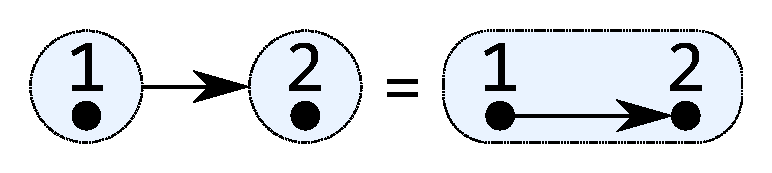
\includegraphics[scale=0.27]{fig/ex-b.pdf}}
\vspace{-2.4mm}
\caption{$1 \rightarrow 2$}
\end{subfigure}
\hspace{11mm}
\begin{subfigure}[b]{0.17\linewidth}
\centerline{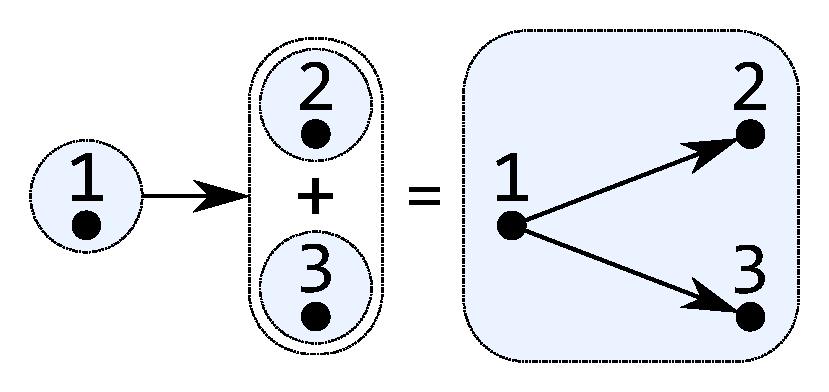
\includegraphics[scale=0.27]{fig/ex-c.pdf}}
\vspace{-1mm}
\caption{$1 \rightarrow (2 + 3)$}
\end{subfigure}
\hspace{12mm}
\begin{subfigure}[b]{0.15\linewidth}
\centerline{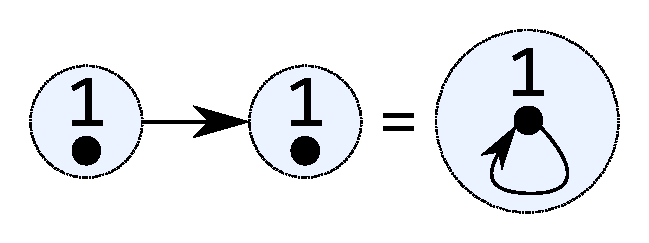
\includegraphics[scale=0.27]{fig/ex-d.pdf}}
\vspace{2.4mm}
\caption{$1 \rightarrow 1$}
\end{subfigure}
\hspace{12mm}
\begin{subfigure}[b]{0.2\linewidth}
\centerline{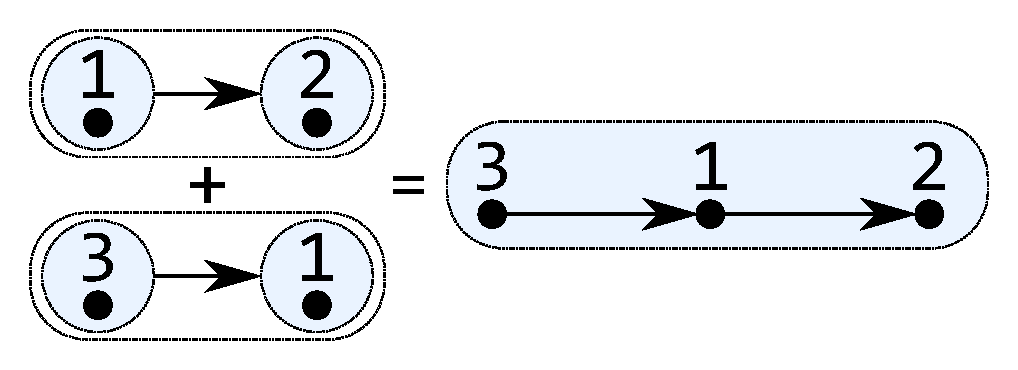
\includegraphics[scale=0.27]{fig/ex-e.pdf}}
\vspace{-1mm}
\caption{$1 \rightarrow 2 + 3 \rightarrow 1$}
\end{subfigure}
\vspace{-1mm}
\caption{Examples of graph construction\label{fig-construction}}
\vspace{-3mm}
\end{figure}

\vspace{-1mm}
\subsection{Type class}\label{sub-class}

We abstract the graph construction primitives defined in \S\ref{sub-constructing}
as the type class \hs{Graph}:

\begin{minted}{haskell}
class Graph g where
    type Vertex g
    empty   :: g
    vertex  :: Vertex g -> g
    overlay :: g -> g -> g
    connect :: g -> g -> g
\end{minted}

\noindent
Here the associated type\footnote{Associated
types~\cite{2005_associated_type_chakravarty} require the \textsf{TypeFamilies}
GHC extension.} \hs{Vertex@\,@g} corresponds to the universe of graph
vertices $\mathbb{V}$, \hs{empty} is the empty graph
$\varepsilon$, \hs{vertex} constructs a graph with a single vertex,
and \hs{overlay} and \hs{connect} compose given graphs according to
the definitions in~\S\ref{sub-constructing}. All methods of the type class
are total, i.e. are defined for all possible inputs, therefore,
the presented API allows \emph{fewer opportunities for usage errors}
and \emph{greater opportunities for reuse}.

Let's put the API to the test and construct some graphs! A single edge is
obtained by connecting two vertices:

\begin{minted}{haskell}
edge :: Graph g => Vertex g -> Vertex g -> g
edge x y = connect (vertex x) (vertex y)
\end{minted}

\noindent
The graphs in Fig.~\ref{fig-construction}(b,d) are \hs{edge@\,@1@\,@2} and
\hs{edge@\,@1@\,@1}, respectively.
A graph that contains a given list of isolated vertices can be constructed
as follows:

\begin{minted}{haskell}
vertices :: Graph g => [Vertex g] -> g
vertices = @\std{foldr}@ overlay empty . @\std{map}@ vertex
\end{minted}

\noindent
That is, we turn each vertex into a singleton graph and overlay the results.
The graph in Fig.~\ref{fig-construction}(a) is \hs{vertices@\,@[1,2]}.
By replacing \hs{overlay} with \hs{connect} in the above
function, we obtain a \emph{clique} -- a fully connected graph on a given list
of vertices:

\begin{minted}{haskell}
clique :: Graph g => [Vertex g] -> g
clique = @\std{foldr}@ connect empty . @\std{map}@ vertex
\end{minted}

\noindent
For example, the infinite clique on all positive integers is \hs{clique@\,@[1..]}.

The above graph construction functions are total, fully polymorphic, and elegant.
Thanks to the minimalistic core type class, it is easy to wrap your favourite
graph library into the described interface, and reuse these functions, as well
as many others that we define throughout this paper.

\section{Algebraic structure}\label{sec-algebra}

The functions \hs{edge}, \hs{vertices} and \hs{clique} defined in the previous
section \S\ref{sec-core} satisfy a few properties that we can intuitively write down,
but which may seem tricky to prove (we encourage the reader to try):
\begin{itemize}
    \item \hs{vertex x} $\ =\ $ \hs{vertices [x]} and \hs{edge x y} $\ =\ $ \hs{clique [x,y]}.
    \item \hs{vertices xs} $\ \subseteq\ $ \hs{clique xs}, where $x \subseteq y$ means
    $x$ is a subgraph of $y$.
    \item \hs{clique (xs ++ ys)} $\ =\ $ \hs{connect (}\hs{clique xs) (}\hs{clique ys)}.
\end{itemize}

In this section we characterise the \hs{Graph} type class with a set of
axioms that reveal an algebraic structure very similar to a semiring\footnote{
See Dolan~\citeyear{2013_semirings_dolan} for an entertaining exploration of
applications of semirings in graph theory.}.
This provides a convenient framework for proving the above properties using equational
reasoning, and is generally useful for formal verification, as well as automated testing
of graph library APIs, e.g. by using QuickCheck~\cite{2011_quickcheck_claessen}.

\begin{figure}
\begin{subfigure}[b]{0.4\linewidth}
\centerline{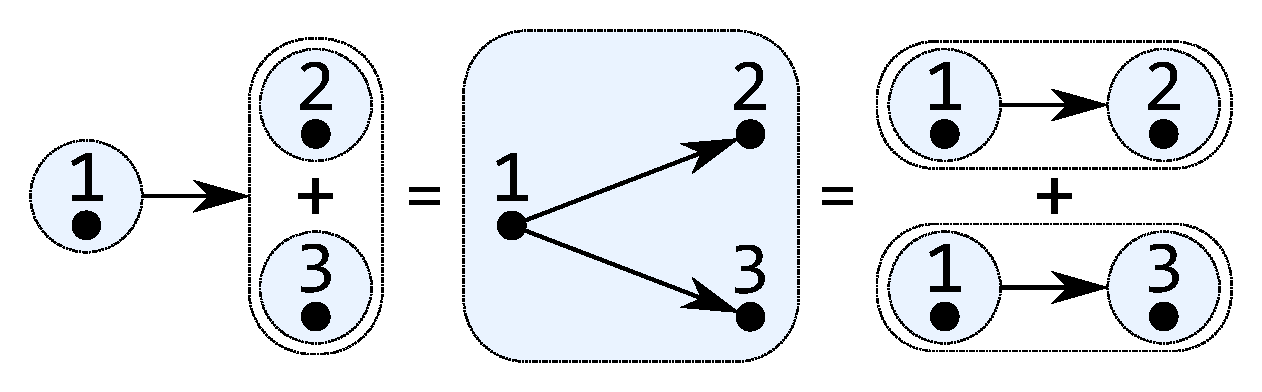
\includegraphics[scale=0.27]{fig/ax-distributivity.pdf}}
\caption{Distributivity: $1 \rightarrow (2 + 3) = 1 \rightarrow 2 + 1 \rightarrow 3$ }
\end{subfigure}
\hspace{12mm}
\begin{subfigure}[b]{0.5\linewidth}
\centerline{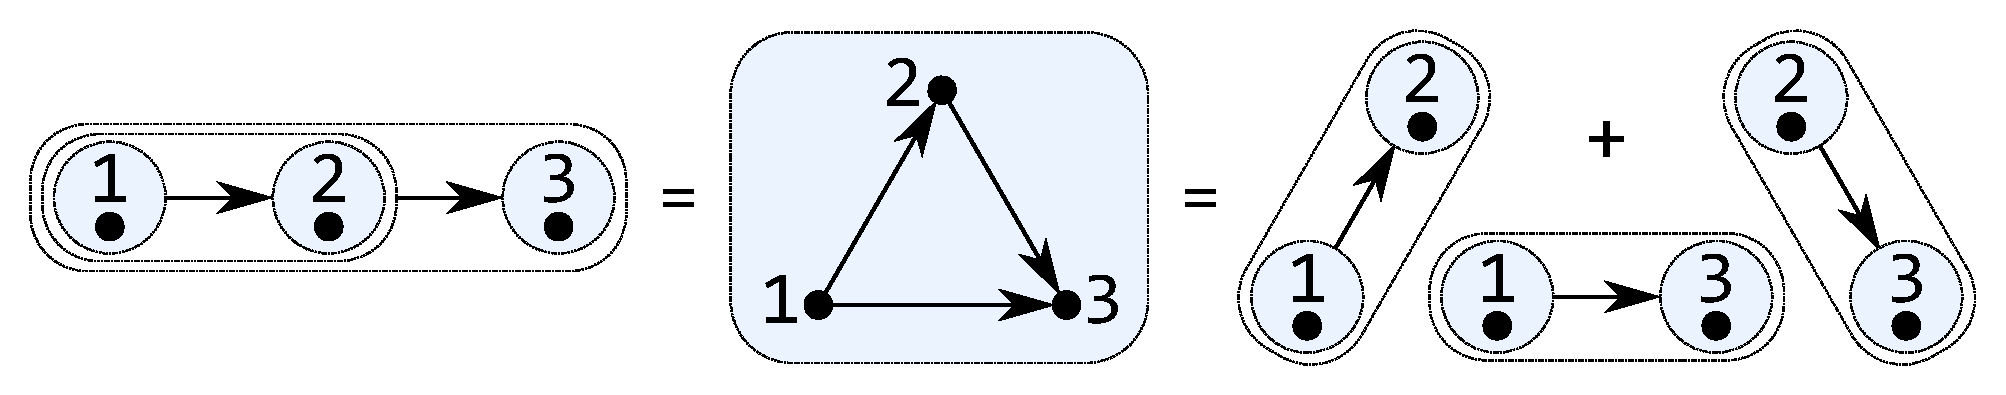
\includegraphics[scale=0.27]{fig/ax-decomposition.pdf}}
\caption{Decomposition: $1 \rightarrow 2 \rightarrow 3 = 1 \rightarrow 2 +
1 \rightarrow 3 + 2 \rightarrow 3$}
\end{subfigure}
\vspace{-3mm}
\caption{Two axioms of the algebra of graphs\label{fig-axioms}}
\vspace{-4mm}
\end{figure}

\subsection{Axiomatic characterisation}

The definitions of \hs{vertices} and \hs{clique} in \S\ref{sub-class}
use $\varepsilon$ as the identity for both overlay $+$ and connect $\rightarrow$
operations. This seems unusual, but we can easily check that
$x + \varepsilon = x$ and $x \rightarrow \varepsilon = x$ for any graph $x \in G$
by plugging the empty graph into the definitions of overlay and connect,
respectively. Furthermore, we can verify the following:
\begin{itemize}
    \item $(G,+,\varepsilon)$ is an idempotent commutative monoid.
    \item $(G,\rightarrow,\varepsilon)$ is a monoid.
    \item $\rightarrow$ distributes over $+$, e.g.
    $1 \rightarrow (2 + 3) = 1 \rightarrow 2 + 1 \rightarrow 3$, as illustrated
    in Fig.~\ref{fig-axioms}(a).
\end{itemize}

\noindent
The above looks remarkably close to a semiring, with the only oddity being the shared
identity of the two operations. The following \emph{decomposition} law is
what makes the algebra of graphs different:
\[
x \rightarrow y \rightarrow z = x \rightarrow y + x \rightarrow z + y \rightarrow z
\]

\noindent
Fig.~\ref{fig-axioms}(b) illustrates the law by showing that the triangle
graph can be obtained in two different ways: by connecting three vertices
of the triangle or by constructing its edges separately and overlaying them.

Interestingly, the fact that overlay and connect share the same identity
follows from the decomposition law. Indeed, let $\varepsilon_{+}$ and
$\varepsilon_{\rightarrow}$ stand for the identities of $+$ and $\rightarrow$,
respectively. Then:
\[
\begin{array}{rcll}
\varepsilon_{+} & = & \varepsilon_{+} \rightarrow \varepsilon_{\rightarrow} \rightarrow \varepsilon_{\rightarrow} & \text{(identity of $\rightarrow$)}\\
 & = & \varepsilon_{+} \rightarrow \varepsilon_{\rightarrow} + \varepsilon_{+} \rightarrow \varepsilon_{\rightarrow} + \varepsilon_{\rightarrow} \rightarrow \varepsilon_{\rightarrow} & \text{(decomposition)}\\
 & = & \varepsilon_{+} + \varepsilon_{+} + \varepsilon_{\rightarrow} & \text{(identity of $\rightarrow$)}\\
 & = & \varepsilon_{\rightarrow} & \text{(identity of $+$)}\\
\end{array}
\]

\noindent
Furthermore, the idempotence of $+$ also follows from the decomposition, which
leads to the following \emph{minimal set of axioms that characterise algebraic graphs}:

\begin{itemize}
    \item $+$ is commutative and associative: $x + y = y + x$ and
    $x + (y + z) = (x + y) + z$.
    \item $(G, \rightarrow, \varepsilon)$ is a monoid:
    $\varepsilon \rightarrow x = x \rightarrow \varepsilon = x$ and
    $x \rightarrow (y \rightarrow z) = (x \rightarrow y) \rightarrow z$.
    \item Distributivity:
    $x \rightarrow (y + z) = x \rightarrow y + x \rightarrow z$ and
    $(x + y) \rightarrow z = x \rightarrow z + y \rightarrow z$.
    \item Decomposition: $x \rightarrow y \rightarrow z =
    x \rightarrow y + x \rightarrow z + y \rightarrow z$.
\end{itemize}

We require all \hs{Graph} instances to satisfy these 8 axioms. Our definition
of graph construction primitives in~\S\ref{sub-constructing} does satisfy them
all and is therefore a valid \hs{Graph} instance, which we will implement
in~\S\ref{sub-instances}. There are many other useful instances and we will discuss
them in~\S\ref{sec-a-la-carte}. Some of them satisfy additional
axioms, for example, by making the connect $\rightarrow$ operation commutative,
we obtain undirected graphs.

Algebraic graphs are \emph{complete} in the sense that it is possible to describe
any graph using the core interface. Indeed, given a graph $(V,E)$ we can construct
it as \hs{graph@$\,V\,E$@} where function \hs{graph} is defined as follows.

\begin{minted}{haskell}
graph :: Graph g => [Vertex g] -> [(Vertex g, Vertex g)] -> g
graph vs es = overlay (vertices vs) (edges es)
\end{minted}

Here \hs{edges} is a generalisation of \hs{edge} to a list of edges, so that
\hs{edge x y} $\ =\ $ \hs{edges [(x,y)]}:

\begin{minted}{haskell}
edges :: Graph g => [(Vertex g, Vertex g)] -> g
edges = @\std{foldr}@ overlay empty . @\std{map}@ (@\std{uncurry}@ edge)
\end{minted}

Note that \hs{graph} is total thanks to the \emph{absorption theorem}
$x \rightarrow y + x + y = x \rightarrow y$, which in particular states that
an edge $(u,v)$ contains its two vertices $\{u,v\}$ and is inseparable
from them. Therefore, if the pair $(V,E)$ is inconsistent, the set of vertices of
the resulting graph will be expanded to $\hat{V}$ so that
$E\subseteq \hat{V}\times \hat{V}$ holds. More generally,
in addition to being complete, the algebraic graph API is also \emph{sound} in
the sense that it is impossible to construct an inconsistent pair $(V,E)$
using the four \hs{Graph} methods.

The following theorems can be proved from the minimal set of axioms:

\begin{itemize}
    \item Identity of $+$: $x + \varepsilon = x$.
    \item Idempotence of $+$: $x + x = x$.
    \item Absorption: $x \rightarrow y + x + y = x \rightarrow y$.
    \item Saturation: $x \rightarrow x \rightarrow x = x \rightarrow x$.
\end{itemize}

We leave the proof to the reader as a not entirely trivial exercise.
A machine-assisted proof can be found in~\cite{2014_alekseyev_phd}
where the algebra of parameterised graphs (that we build on) has been formalised in Agda.

\subsection{Equational reasoning}\label{sub-reasoning}

We now use the

\subsection{Two \hs{Graph} instances}\label{sub-instances}

free model

\subsection{Automated testing}\label{sub-testing}

arbitrary

\section{Graphs \`{a} la carte}\label{sec-a-la-carte}

\section{Graph transformation library}\label{sec-transformations}

\section{Applications}\label{sec-applications}

\section{Related work}\label{sec-related}

% In this section we review existing approaches to working with graphs developed
% by the functional programming community.

% \begin{itemize}
%     \item Tying the knot:
%     \item Borrowing imperative algorithms via the State monad.
%     \item Data.Graph by King & Launchbury, 1995. \url{https://galois.com/wp-content/uploads/2014/08/pub_JL_StructuringDFSAlgorithms.pdf}.
%     Clever tricks exploiting lazy evaluation (Johnsson 1998) \url{https://pdfs.semanticscholar.org/a6ed/4e55f148e0c48445269990102838f7d7abb5.pdf?_ga=1.176470501.1134931652.1487554701}

%     \item Inductive Graphs by Martin Erwig, 2001. \url{https://web.engr.oregonstate.edu/~erwig/papers/InductiveGraphs_JFP01.pdf}
%     \item Structured Graphs by Oliveira & Cook. \url{https://www.cs.utexas.edu/~wcook/Drafts/2012/graphs.pdf}
%     \item An initial-algebra approach to directed acyclic graphs, by J. Gibbons
%     \item "Algebras for graphs have been studied in the context of graph rewriting, see Bauderon and Courcelle (1986), for example."
% \end{itemize}

\section{Discussion and future work}\label{sec-discussion}

% Using discrimination library for better efficiency
% Modular decomposition for minimisation
% Solving graph equations


%% Acknowledgments
\begin{acks}                            %% acks environment is optional
                                        %% contents suppressed with 'anonymous'
  %% Commands \grantsponsor{<sponsorID>}{<name>}{<url>} and
  %% \grantnum[<url>]{<sponsorID>}{<number>} should be used to
  %% acknowledge financial support and will be used by metadata
  %% extraction tools.
  This material is based upon work supported by the
  \grantsponsor{GS100000001}{National Science
    Foundation}{http://dx.doi.org/10.13039/100000001} under Grant
  No.~\grantnum{GS100000001}{nnnnnnn} and Grant
  No.~\grantnum{GS100000001}{mmmmmmm}.  Any opinions, findings, and
  conclusions or recommendations expressed in this material are those
  of the author and do not necessarily reflect the views of the
  National Science Foundation.
\end{acks}

\bibliography{publications}

% \appendix
% \section{Appendix}

% Text of appendix \ldots

\end{document}
